\section{光滑点与奇异点}\label{sec:smooth-and-singular-points}

切空间最重要的用途之一是检测仿射簇是否有\textquotedbl{}折角\textquotedbl{}或\textquotedbl{}尖点\textquotedbl{}. 例如, 如 Example~\ref{ex:linearizations-of-cusp} 所见, 簇 $\mathcal{V}(x^{2}-y^{3})\subseteq\mathbb{A}^{2}$ 的\textquotedbl{}尖点\textquotedbl{}很特殊: 该点的切空间是二维的, 而其余各点的切空间都是一维的. 簇中切空间维数发生跳跃的这些特殊点称为奇异点, 下面给出精确定义.

\begin{Definition}{光滑点与奇异点}\leavevmode\label{def:smooth-and-singular-points}
设 $X$ 为不可约仿射簇, 且 $a\in X$. 若 $\dim(T_{a}X)=\dim(X)$, 则称 $X$ 在 $a$ 处\emph{光滑}; 否则称 $X$ 在 $a$ 处\emph{奇异}. 若 $X$ 在每一点 $a\in X$ 处都光滑, 则称 $X$ \emph{光滑}; 否则称 $X$ \emph{奇异}.
\end{Definition}

\BookPairedNoteLeft
  {也可以定义可约簇的光滑性. 但由于不同分支的维数可能不同, 应把 $X$ 的维数换成它在 $a$ 处的局部维数, 即所有包含 $a$ 的不可约分支的维数的最大值.}
  {由 Proposition~\ref{prop:tangent-dimension-lower-bound}, 奇异点就是满足 $\dim(T_{a}X)>\dim(X)$ 的点 $a\in X$.}
为简单起见, 关于光滑性的整个讨论只限于不可约簇.

\begin{Example}{仿射空间是光滑的}\leavevmode\label{ex:affine-space-is-smooth}
由于 $\mathcal{I}(\mathbb{A}^{n})=\{0\}\subseteq K[x_{1},\ldots,x_{n}]$, 对任意 $a\in\mathbb{A}^{n}$ 有
\[
  L_{a}\mathbb{A}^{n}=\mathcal{V}(L_{a}0)=\mathcal{V}(0)=\mathbb{A}^{n},
\]
这蕴含 $T_{a}\mathbb{A}^{n}=K^{n}$. 因此
\[
  \dim(T_{a}\mathbb{A}^{n})=\dim(K^{n})=n=\dim(\mathbb{A}^{n}),
\]
说明 $\mathbb{A}^{n}$ 在所有点处都光滑.
\end{Example}

\begin{Example}{尖点曲线在原点处奇异}\leavevmode\label{ex:cusp-singular-at-origin}
考虑 Examples~\ref{ex:linearizations-of-cusp} 和~\ref{ex:tangent-space-of-cusp} 中的簇 $X=\mathcal{V}(x^{2}-y^{3})\subseteq\mathbb{A}^{2}$. 切空间 $T_{a}X$ 在 $a=(0,0)$ 时是二维的, 而在 $X$ 的其余各点处是一维的. 由于 $X$ 本身是一维簇, 这说明 $X$ 在原点处奇异, 但在其余各点处光滑.
\end{Example}

\begin{Example}{锥面是奇异的}\leavevmode\label{ex:cone-singular-at-origin}
\BookPairedFigure
  {令 $X=\mathcal{V}(x^{2}+y^{2}-z^{2})\subseteq\mathbb{A}^{3}_{\mathbb{C}}$, 即\hyperref[fig:singular-cone-real-points]{右图}画出实点的锥面. 可以证明 $X$ 在原点处奇异, 此处曲面收缩成一点; 而在其余各点处光滑 (Exercise~\ref{ex:complex-cone-smooth-except-at-origin}).}
  {\phantomsection\label{fig:singular-cone-real-points}%
   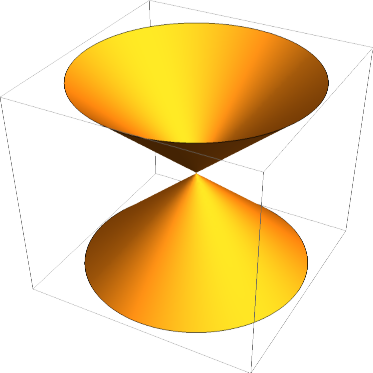
\includegraphics[width=\linewidth]{figures/singular-cone.png}}
\end{Example}

由于仿射簇 $X\subseteq\mathbb{A}^{n}$ 的切空间是 $K^{n}$ 的向量子空间, 自然会预期可用线性代数的工具确定簇的奇异点. 将线性代数工具用于研究切空间和奇异性所需的关键对象是 Jacobian 矩阵. 它只是把有限个多项式的偏导数排成矩阵.

\begin{Definition}{Jacobian 矩阵}\leavevmode\label{def:jacobian-matrix}
给定多项式 $f_{1},\ldots,f_{m}\in K[x_{1},\ldots,x_{n}]$, $f_{1},\ldots,f_{m}$ 的\emph{Jacobian 矩阵}是 $m\times n$ 矩阵
\[
  \operatorname{Jac}_{f_{1},\ldots,f_{m}}=
  \begin{pmatrix}
    \dfrac{\partial f_{1}}{\partial x_{1}} & \cdots & \dfrac{\partial f_{1}}{\partial x_{n}}\\
    \vdots & \ddots & \vdots\\
    \dfrac{\partial f_{m}}{\partial x_{1}} & \cdots & \dfrac{\partial f_{m}}{\partial x_{n}}
  \end{pmatrix}.
\]
\end{Definition}

注意矩阵 $\operatorname{Jac}_{f_{1},\ldots,f_{m}}$ 的元素都属于 $K[x_{1},\ldots,x_{n}]$, 所以可以在任一点 $a\in\mathbb{A}^{n}$ 处取值, 得到 $m\times n$ 矩阵
\[
  \operatorname{Jac}_{f_{1},\ldots,f_{m}}(a)\in K^{mn}.
\]
下一个结果将 $a$ 处的切空间解释为一个 Jacobian 矩阵的核, 由此可用行列式刻画簇的奇异点.

\begin{Proposition}{光滑性的 Jacobian 判据}\leavevmode\label{prop:jacobian-criterion-for-smoothness}
若 $X\subseteq\mathbb{A}^{n}$ 是不可约仿射簇, 且 $\mathcal{I}(X)=\langle f_{1},\ldots,f_{m}\rangle$, 则
\[
  T_{a}X=\ker(\operatorname{Jac}_{f_{1},\ldots,f_{m}}(a)).
\]
因此, $X$ 在 $a\in X$ 处奇异当且仅当
\[
  \operatorname{rk}(\operatorname{Jac}_{f_{1},\ldots,f_{m}}(a))<\operatorname{codim}(X).
\]
\end{Proposition}
\begin{Proof}
注意 $\operatorname{Jac}_{f_{1},\ldots,f_{m}}(a)$ 的各行是函数 $f_{1},\ldots,f_{m}$ 的梯度:
\[
  \operatorname{Jac}_{f_{1},\ldots,f_{m}}(a)=
  \begin{pmatrix}
    \nabla f_{1}(a)\\
    \vdots\\
    \nabla f_{m}(a)
  \end{pmatrix}.
\]
由矩阵乘法的定义, $v\in\ker(\operatorname{Jac}_{f_{1},\ldots,f_{m}}(a))$ 当且仅当对所有 $i=1,\ldots,m$ 都有 $\nabla f_{i}(a)\cdot v=0$. 所以由 Proposition~\ref{prop:gradient-characterization-of-tangent-spaces} 及其证明之后紧接的说明可知
\[
  T_{a}X=\ker(\operatorname{Jac}_{f_{1},\ldots,f_{m}}(a)).
\]
秩--零度定理于是蕴含
\[
  \dim(T_{a}X)=n-\operatorname{rk}(\operatorname{Jac}_{f_{1},\ldots,f_{m}}(a)).
\]
由 Proposition~\ref{prop:tangent-dimension-lower-bound} 可得
\[
  \operatorname{rk}(\operatorname{Jac}_{f_{1},\ldots,f_{m}}(a))\leq\operatorname{codim}(X),
\]
再由光滑点和奇异点的定义, $X$ 在 $a$ 处奇异当且仅当等号不成立.
\end{Proof}

在超曲面的情形, Jacobian 判据特别简单.

\begin{Example}{超曲面的 Jacobian 判据}\leavevmode\label{ex:jacobian-criterion-for-hypersurfaces}
令 $X=\mathcal{V}(f)$, 其中 $f\in K[x_{1},\ldots,x_{n}]$ 不可约, 于是 $\mathcal{I}(X)=\langle f\rangle$. 那么 $\operatorname{codim}(X)=1$, 而 Jacobian 判据表明, $X$ 在 $a$ 处奇异当且仅当 $1\times n$ 矩阵
\[
  \left(\frac{\partial f}{\partial x_{1}}(a)\quad\cdots\quad
    \frac{\partial f}{\partial x_{n}}(a)\right)
\]
的秩为零. 因此 $X$ 在 $a$ 处奇异当且仅当
\[
  \frac{\partial f}{\partial x_{1}}(a)=\cdots=\frac{\partial f}{\partial x_{n}}(a)=0.
\]
\end{Example}

由 Proposition~\ref{prop:jacobian-criterion-for-smoothness}, 簇的奇异点由 Jacobian 矩阵降秩的点刻画. 这一刻画有一个便利的性质: Jacobian 矩阵降秩的点本身就是一组多项式方程的解. 由此得到下面的重要结论.

\begin{Corollary}{奇异点集是闭的}\leavevmode\label{cor:singular-locus-is-closed}
若 $X\subseteq\mathbb{A}^{n}$ 为不可约仿射簇, 且 $\operatorname{Sing}(X)\subseteq X$ 是 $X$ 的奇异点集, 则 $\operatorname{Sing}(X)$ 也是仿射簇.
\end{Corollary}

在给出证明之前, 先回忆: 矩阵 $M$ 的一个 $r\times r$ 子式, 是从 $M$ 删去若干行和列后得到的 $r\times r$ 矩阵的行列式. 线性代数的一个重要结论指出, $\operatorname{rk}(M)<r$ 当且仅当 $M$ 的所有 $r\times r$ 子式都为零.

\begin{Proof}\textbf{of Corollary~\ref{cor:singular-locus-is-closed}.}\quad
选取一组生成元 $\mathcal{I}(X)=\langle f_{1},\ldots,f_{m}\rangle$, 并为简便起见令 $r=\operatorname{codim}(X)$. 由 Proposition~\ref{prop:jacobian-criterion-for-smoothness}, 点 $a\in\mathbb{A}^{n}$ 是 $X$ 的奇异点当且仅当对所有 $i=1,\ldots,m$, $f_{i}(a)=0$, 且
\[
  \operatorname{rk}(\operatorname{Jac}_{f_{1},\ldots,f_{m}}(a))<r.
\]
所以 $\operatorname{Sing}(X)$ 是多项式 $f_{1},\ldots,f_{m}\in K[x_{1},\ldots,x_{n}]$ 和 $\operatorname{Jac}_{f_{1},\ldots,f_{m}}$ 的 $r\times r$ 子式的共同零点集, 其中每个子式都是 $K[x_{1},\ldots,x_{n}]$ 中的多项式.
\end{Proof}

知道 $\operatorname{Sing}(X)$ 是仿射簇后, 就可以用研究仿射簇的所有工具来研究 $\operatorname{Sing}(X)$. 例如可以计算 $\operatorname{Sing}(X)$ 的维数. 下一个例子说明, 不可约超曲面上的\textquotedbl{}几乎所有点\textquotedbl{} (在维数论意义下) 都是光滑点.

\begin{Example}{不可约超曲面的泛光滑性}\leavevmode\label{ex:generic-smoothness-of-irreducible-hypersurfaces}
设 $X=\mathcal{V}(f)\subseteq\mathbb{A}^{n}$, 其中 $f\in K[x_{1},\ldots,x_{n}]$ 不可约. 我们断言 $X$ 至少有一个光滑点. 为论证这一点, 反设 $X$ 的每一点都是奇异点. 由 Jacobian 判据, 这意味着
\[
  \frac{\partial f}{\partial x_{1}},\ldots,\frac{\partial f}{\partial x_{n}}
     \in K[x_{1},\ldots,x_{n}]
\]
都在 $X$ 上取值为零, 所以它们属于消没理想 $\mathcal{I}(X)=\langle f\rangle$. 由于 $f$ 不可约, 它不可能是常数. 不妨假设 $f$ 关于 $x_{1}$ 有正次数. 那么 $\partial f/\partial x_{1}$ 不是零多项式, 且关于 $x_{1}$ 的次数严格小于 $f$ 的次数, 与其属于 $\langle f\rangle$ 矛盾.

因此 $X$ 至少有一个光滑点, 从而 $\operatorname{Sing}(X)\subsetneq X$. 既然 $\operatorname{Sing}(X)$ 和 $X$ 都是仿射簇, 且 $X$ 不可约, 由 Proposition~\ref{prop:dimension-monotonicity} 得 $\dim(\operatorname{Sing}(X))<\dim(X)$. 换句话说, 由于 $\operatorname{Sing}(X)$ 的维数严格小于 $X$ 的维数, 奇异点形成 $X$ 中很特殊的一个点集: $X$ 的几乎所有点都是光滑点. 这一性质常称为\emph{泛光滑性}.
\end{Example}

注意, 泛光滑性对一般的仿射簇也成立. 这由每个仿射簇至少有一个光滑点这一事实推出. 这个一般事实的证明略超出目前讨论的范围.

\BookExerciseHeading
\begin{BookExercises}
  \item\label{ex:smoothness-is-intrinsic} 证明光滑性是仿射簇的内在性质.
  \item\label{ex:singularities-of-nodal-cubic} 考虑仿射簇 $X=\mathcal{V}(y^{2}-x^{3}-x^{2})\subseteq\mathbb{A}^{2}_{\mathbb{C}}$.
  \begin{enumerate}
    \item 画出 $X$ 的实点, 并猜测 $X$ 可能在哪些点处奇异.
    \item 用 Jacobian 判据求出 $X$ 奇异的所有点.
  \end{enumerate}
  \item\label{ex:smooth-affine-double-cover-of-square-free-polynomial} 设 $f\in K[x_{1},\ldots,x_{n}]$ 为无平方因子的多项式, 考虑仿射簇 $X=\mathcal{V}(x_{n+1}^{2}-f)\in\mathbb{A}^{n+1}$.
  \begin{enumerate}
    \item 证明 $X$ 不可约.
    \item 证明 $X$ 光滑.
  \end{enumerate}
  \item\label{ex:complex-unit-sphere-is-smooth} 证明复单位球面 $X=\mathcal{V}(x_{1}^{2}+\cdots+x_{n}^{2}-1)\subseteq\mathbb{A}_{\mathbb{C}}^{n}$ 光滑.
  \item\label{ex:complex-cone-smooth-except-at-origin} 证明复锥面 $\mathcal{V}(x^{2}+y^{2}-z^{2})\subseteq\mathbb{A}^{3}_{\mathbb{C}}$ 在原点处奇异, 在其余各点处光滑.
  \item\label{ex:singular-points-of-whitney-umbrella} 求 Whitney 伞 $\mathcal{V}(x^{2}+y^{2}z)\subseteq\mathbb{A}^{3}$ 的所有奇异点. (Whitney 伞的实点见 Example~\ref{ex:singleton-vanishing-sets} 中的图.)
  \item\label{ex:jacobian-smoothness-of-affine-twisted-cubic} 考虑仿射扭三次曲线 $X=\mathcal{V}(y-x^{2},z-x^{3})\subseteq\mathbb{A}^{3}$. 已知 $X\cong\mathbb{A}^{1}$, 因而 $X$ 光滑. 用 Jacobian 判据给出另一个光滑性证明.
\end{BookExercises}
